\section{Execution}
\label{sec:Durchführung}

\begin{figure}
    \centering 
    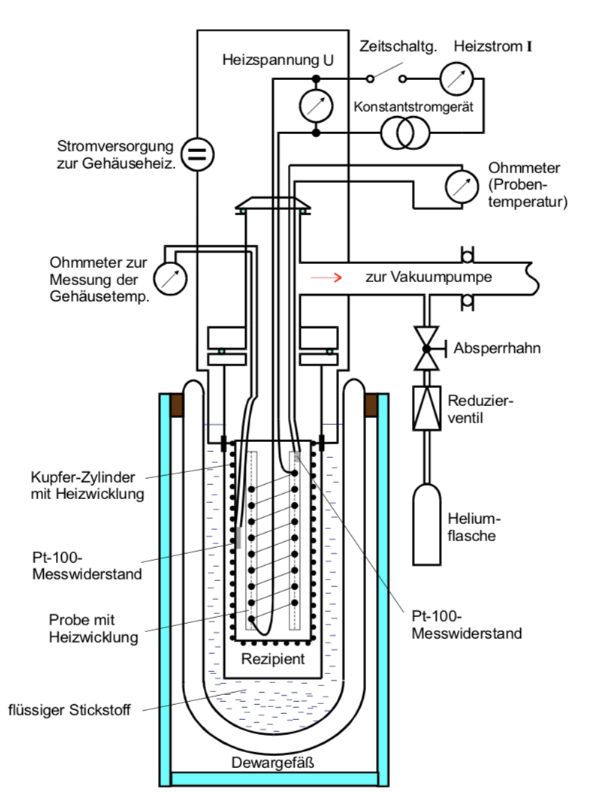
\includegraphics[width=.8\textwidth]{Bilder/Aufbau.PNG}
    \caption{Experimental setup. \cite{V47}}
    \label{fig:Aufbau}
\end{figure}


The used experimental setup is shown in figure \ref{fig:Aufbau}.
At first the rezipient has to be vaccuated and be filled by heliumgas.
The sample ($m=\SI{342}{\g}$) in this rezipient is surrondend by liquid nitrogen, to cool the sample on nearly $T=\SI{80}{\kelvin}$. 
The liquid nitrogen is filled in a dewar vessel and is kept there through the whole prozess.
To heat the copper with a given value there is a heating coil with a adjustable engergy input.
The added engergy depends on the current and the voltage.
To reduce heat losses through other channels like radiation or convektion, the rezipient is kept at the same temperature as the sample.
The temperature is messured indirectly by Pt-100-resistors.
To calculate the temperatures the equation
\begin{equation}
    T = 0.00134 R^2 + 2.296 R - 243.02
\end{equation}
is used.
$R$ is the messured resistance.




Starting by a temperature of $T=\SI{-180}{\celsius}$, the temperature is raised evenly till $T=\SI{20}{\celsius}$. 
The temperature, respectively the resistances, the time and the current is messured and noted past every $\SI{10}{\kelvin}$.
%Was wurde gemessen bzw. welche Größen wurden variiert?